
\subsection{Matriz de adyacencia}
\label{sec:matriz_de_adyacencia}

Una forma de representar un grafo es utilizar una matriz donde el índice de cada fila y de cada columna representa un vértice del grafo, de forma que una casilla de la matriz representan si existe o no un arco entre el vértice representado por la fila y el representado por la columna.

\begin{definicion}{Matriz de adyacencia}{matriz_de_adyacencia}
  Sea \(G\) un grafo simple, con vértices \(v_0, \ldots, v_{n-1}\), la \concept{matriz de adyacencia} de \(G\) es una matriz cuadrada \(\bmat{A}\) de tamaño \(n\times n\) tal que si \(v_i \longrightarrow v_j\), entonces \(a_{ij} = 1\) y si \(v_i \not\longrightarrow v_j\), entonces el valor de \(a_{ij} = 0\).
\end{definicion}

Si \(G\) es además ponderado, entonces cada elemento de la matriz representa el peso del respectivo arco, de forma que si \(v_i \longrightarrow v_j\), entonces \(a_{ij} = w(v_i, v_j)\).

\begin{center}
  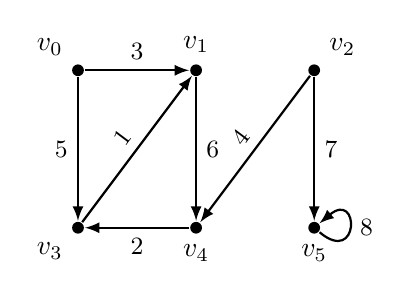
\begin{tikzpicture}[baseline=(current bounding box.center),
    vertex/.style={circle, fill=black, inner sep=1.5pt},
    -latex, thick,
  ]
    \node[vertex, label=above left:\(v_0\)]  (v0) at (0, 2)   {};
    \node[vertex, label=above:\(v_1\)]       (v1) at (1.5, 2) {};
    \node[vertex, label=above right:\(v_2\)] (v2) at (3, 2)   {};
    \node[vertex, label=below left:\(v_3\)]  (v3) at (0, 0)   {};
    \node[vertex, label=below:\(v_4\)]       (v4) at (1.5, 0) {};
    \node[vertex, label=below:\(v_5\)]       (v5) at (3, 0)   {};

    \draw (v0) -- (v1) node[midway, above] {\small 3};
    \draw (v0) -- (v3) node[midway, left] {\small 5};
    \draw (v3) -- (v1) node[midway, above, sloped] {\small 1};
    \draw (v1) -- (v4) node[midway, right] {\small 6};
    \draw (v4) -- (v3) node[midway, below] {\small 2};
    \draw (v2) -- (v4) node[midway, above, sloped] {\small 4};
    \draw (v2) -- (v5) node[midway, right] {\small 7};
    \draw (v5) to[out=-40, in=40, looseness=15] node[right] {\small 8} (v5);
  \end{tikzpicture}
  \hspace{1.5cm}
  \(
  \begin{pmatrix}
    0 & 3 & 0 & 5 & 0 & 0 \\
    0 & 0 & 0 & 0 & 6 & 0 \\
    0 & 0 & 0 & 0 & 4 & 7 \\
    0 & 1 & 0 & 0 & 0 & 0 \\
    0 & 0 & 0 & 2 & 0 & 0 \\
    0 & 0 & 0 & 0 & 0 & 8
  \end{pmatrix}
  \)
  \captionof{figure}{Un grafo dirigido, ponderado y disperso junto a su matriz de adyacencia.}
  \label{fig:matriz_de_adyacencia}
\end{center}

\subsubsection{Ventajas}
\label{sec:ventajas}

La gran ventaja de la matriz de adyacencia es que es óptima para toda operación que se realice sobre una sola arista del grafo, pues esas operaciones suponen simplemente cambiar un valor en la matriz, con complejidad temporal de \(\Theta(1)\):
\begin{itemize}
  \item Insertar una arista.
  \item Conocer si existe una arista.
  \item Actualizar el peso de una arista.
  \item Eliminar una arista.
\end{itemize}

\subsubsection{Desventajas}
\label{sec:desventajas}

La principal desventaja de la estructura es su complejidad espacial, que siempre es cuadrática respecto al número de vértices, \(\Theta (n^2)\). Esto hace que al representar ciertos grafos se desperdicie mucho espacio.

Si el grafo representado es denso, esa desventaja no es tan pronunciada; pero si es disperso, la matriz es dispersa: está llena de ceros que representan la ausencia de arcos.

Sumado a eso, si el grafo es no dirigido la matriz es simétrica, pues \(v_i \longrightarrow v_j\) si y solamente si \(v_j \longrightarrow v_i\), de forma que \(a_{ij} = a_{ji}\) para cualesquiera \(i\) y \(j\). La parte triangular superior duplica la información de la parte triangular inferior, se hubiese podido utilizar la mitad del espacio para representar la matriz.

Como desventaja adicional, para conocer el grado de un vértice hay que sumar los valores de toda una fila o columna, un costo de \(\Theta(n)\).
